\documentclass[conference]{IEEEtran}
% NOTE: IEEEtran (on CTAN/MiKTeX) is used for a reliably compiling draft; the
% camera-ready ICASSP submission uses the official spconf.sty template, which is
% a drop-in change of \documentclass and title block.

\usepackage{amsmath,amssymb,amsthm}
\usepackage{graphicx}
\usepackage{bm}
\usepackage[hidelinks]{hyperref}
\graphicspath{{figures/}{../results/figures/}}

\newtheorem{theorem}{Theorem}
\newtheorem{proposition}{Proposition}
\newtheorem{lemma}{Lemma}
\newtheorem{corollary}{Corollary}
\newtheorem{definition}{Definition}

\DeclareMathOperator{\curl}{curl}
\DeclareMathOperator{\rank}{rank}
\DeclareMathOperator{\tr}{tr}
\newcommand{\B}{\bm{B}}
\newcommand{\R}{\mathbb{R}}
\newcommand{\E}{\mathbb{E}}
\newcommand{\Scal}{\mathcal{S}}
\newcommand{\Ttri}{\mathcal{T}}

\begin{document}

\title{When Are Triangles Invisible? Fundamental Limits of\\ Higher-Order Structure Identifiability from Edge Flows}

\author{\IEEEauthorblockN{Anonymous}
\IEEEauthorblockA{Submitted to IEEE ICASSP}}

\maketitle

\begin{abstract}
Topological signal processing models higher-order interactions by placing signals
on the triangles of a simplicial complex, but in many applications the set of
``filled'' triangles is unknown and must be inferred from edge-flow observations.
Existing work provides algorithms for this inference; we instead ask when it is
\emph{possible at all}. We show that the latent higher-order structure is observed
only through the \emph{curl} of the edge flows, which annihilates the gradient and
harmonic parts of the signal. This reduces per-triangle detection to a two-variance
Gaussian test whose optimal error exponent is a Gaussian Chernoff information, and
yields a sharp \emph{curl-invisibility} phase: when the curl signal-to-noise ratio
$\rho$ falls below $\rho^\star(T)=\Theta(\sqrt{\log(1/\delta)/T})$, no estimator can
recover the structure from $T$ snapshots. A geometry-aware whitening of the curl
statistic decorrelates confusable triangles and attains an effective per-triangle
SNR $\rho^{\mathrm{eff}}_\tau=\sigma_c^2/(\sigma_n^2 (\bm{G}^+)_{\tau\tau})$ governed
by the triangle Gram matrix; we prove and empirically confirm a matching
finite-sample recovery law. Finally we expose a second, SNR-independent obstruction:
on a complete graph $K_n$ the curl subspace has dimension $\binom{n-1}{2}$ while
there are $\binom{n}{3}$ candidate triangles, so a $3/n$ fraction is identifiable.
On real daily foreign-exchange flows both obstructions bind: the arbitrage-free
market is curl-free to machine precision, and its complete currency graph exposes
only a third of its triangles. All theorems are validated against Monte-Carlo
simulation; code and data are released for full reproducibility.
\end{abstract}

\begin{IEEEkeywords}
Topological signal processing, simplicial complexes, Hodge decomposition,
identifiability, detection theory, edge flows.
\end{IEEEkeywords}

\section{Introduction}
Graph signal processing captures pairwise structure, but many networked
measurements---currency exchange, traffic circulation, neural flow, statistical
ranking---carry \emph{higher-order} structure that lives on the triangles of a
simplicial complex \cite{barbarossa2020topological,schaub2020random,lim2020hodge}.
Topological signal processing (TSP) has rapidly built a toolbox on the Hodge
Laplacian: convolutional filters \cite{yang2022simplicial}, adaptive
estimation \cite{marinucci2025topological}, unrolled reconstruction
\cite{liu2024unrolling}, and inference of the complex itself from
data \cite{gurugubelli2024simplicial,isufi2025topological}. A recurring primitive is
that the set of filled triangles is unknown and must be learned from edge-flow
signals.

The existing inference methods are \emph{algorithmic}: greedy or sparse-recovery
procedures that return an estimate. None characterizes when the task is
information-theoretically solvable. This paper supplies the missing
\emph{fundamental limits}. Our contributions are:
\begin{enumerate}
\item A \emph{curl-annihilation} reduction (Lemma~\ref{lem:curl}) showing that the
latent structure is observable only through the flow's curl, turning detection into
a two-variance Gaussian test whose error exponent is a Gaussian Chernoff
information (Prop.~\ref{prop:single}).
\item A sharp \emph{curl-invisibility} phase transition
(Theorem~\ref{thm:invis}): the structure is unrecoverable below
$\rho^\star(T)=\Theta(\sqrt{\log(1/\delta)/T})$, with $C(\rho)\!\sim\!\rho^2/16$.
\item A \emph{geometry-aware} whitened detector
(Theorem~\ref{thm:whiten}) with a matching finite-sample recovery law governed by
an effective SNR $\rho^{\mathrm{eff}}_\tau$; it strictly dominates naive
curl-energy thresholding under edge-sharing confusability.
\item An SNR-independent \emph{rank obstruction}
(Theorem~\ref{thm:rank}): on $K_n$ only a $3/n$ fraction of candidate triangles is
identifiable at any SNR.
\end{enumerate}
Every result is validated against Monte-Carlo simulation, and both obstructions are
illustrated on real foreign-exchange flows.

\section{Background and signal model}
\subsection{Hodge structure}
Fix a graph $(\mathcal V,\mathcal E)$ oriented so that the node--edge incidence is
$\B_1\in\R^{|\mathcal V|\times|\mathcal E|}$ and, for a chosen set of filled
triangles, the edge--triangle incidence is $\B_2\in\R^{|\mathcal E|\times|\Ttri|}$.
The boundary-of-boundary identity $\B_1\B_2=\bm 0$ holds, and the Hodge
$1$-Laplacian $\bm L_1=\B_1^{\!\top}\B_1+\B_2\B_2^{\!\top}$ induces the orthogonal
decomposition
\begin{equation}
\R^{|\mathcal E|}=\underbrace{\mathrm{im}\,\B_1^{\!\top}}_{\text{gradient}}\ \oplus\
\underbrace{\mathrm{im}\,\B_2}_{\text{curl}}\ \oplus\
\underbrace{\ker \bm L_1}_{\text{harmonic}} .
\end{equation}
The \emph{curl} of an edge flow is $\curl \bm f=\B_2^{\!\top}\bm f$; a flow induced
by a triangle signal $\bm y$ is $\B_2\bm y$.

\subsection{Generative model}
The $1$-skeleton is known; the latent object is the set $\Scal$ of filled triangles
among a candidate set $\Ttri$ (e.g.\ all $3$-cliques). We observe $T$ i.i.d.\ edge-flow
snapshots
\begin{equation}\label{eq:model}
\bm f_t=\B_1^{\!\top}\bm a_t+\B_{2,\Scal}\,\bm y_t+\bm h_t+\bm n_t,\quad t=1,\dots,T,
\end{equation}
with node potentials $\bm a_t\!\sim\!\mathcal N(\bm 0,\sigma_g^2\bm I)$ (gradient
nuisance), triangle signals $\bm y_t\!\sim\!\mathcal N(\bm 0,\sigma_c^2\bm I)$,
harmonic nuisance $\bm h_t$ and noise $\bm n_t\!\sim\!\mathcal N(\bm 0,\sigma_n^2\bm I)$.
$\B_{2,\Scal}$ keeps the columns of the active triangles. The goal is to recover
$\Scal$ from $\{\bm f_t\}$.

\section{Fundamental limits}
\subsection{Curl annihilation and the single-triangle test}
\begin{lemma}[Curl annihilation]\label{lem:curl}
For any $\bm f$, $\ \B_2^{\!\top}\bm f$ depends only on the curl component:
$\B_2^{\!\top}(\B_1^{\!\top}\bm a)=\bm 0$ and $\B_2^{\!\top}\bm h=\bm 0$ for
$\bm h\in\ker\bm L_1$. Hence under \eqref{eq:model},
$\B_2^{\!\top}\bm f_t=(\B_2^{\!\top}\B_{2,\Scal})\,\bm y_t+\B_2^{\!\top}\bm n_t.$
\end{lemma}
\begin{proof}
$\B_1\B_2=\bm 0$ gives $\B_2^{\!\top}\B_1^{\!\top}=\bm0$. If $\bm L_1\bm h=\bm0$ then
$\bm h^{\!\top}\B_2\B_2^{\!\top}\bm h\le \bm h^{\!\top}\bm L_1\bm h=0$, so
$\B_2^{\!\top}\bm h=\bm0$.
\end{proof}
Thus the gradient and harmonic nuisances---however large---are removed by the curl
map, and only the active triangles and (projected) noise remain.

For an \emph{isolated} candidate triangle $\tau$ (edge-disjoint from other
candidates) the scalar $c_{\tau,t}=\B_{2,\tau}^{\!\top}\bm f_t$ is zero-mean Gaussian
with variance $v_0=3\sigma_n^2$ if $\tau\notin\Scal$ and
$v_1=9\sigma_c^2+3\sigma_n^2$ if $\tau\in\Scal$, since each triangle column has
squared norm $3$.

\begin{proposition}[Two-variance detection]\label{prop:single}
Detecting an isolated $\tau$ from $T$ snapshots is a two-variance Gaussian test.
The energy $E=\sum_t c_{\tau,t}^2$ is a sufficient statistic with $E/v_i\sim\chi^2_T$
under $H_i$, and the minimum Bayes error decays as $\exp(-T\,C(v_0,v_1))$, where
$C(v_0,v_1)=\max_{s\in[0,1]} \tfrac12\!\left[\log(s w_0{+}(1{-}s)w_1)-s\log w_0-(1{-}s)\log w_1\right]$
is the Gaussian Chernoff information, $w_i=1/v_i$.
\end{proposition}

\begin{theorem}[Curl-invisibility phase]\label{thm:invis}
Let $\rho=3\sigma_c^2/\sigma_n^2$, so $v_1=v_0(1+\rho)$. Then $C(\rho)\to0$ as
$\rho\to0$ with $C(\rho)=\rho^2/16+o(\rho^2)$. Consequently, for target error
$\delta$ and budget $T$, reliable detection requires
$\rho\ge\rho^\star(T)=\Theta\!\big(\sqrt{\log(1/\delta)/T}\big)$; below $\rho^\star$
the triangle is unrecoverable by \emph{any} estimator.
\end{theorem}
\begin{proof}[Proof sketch]
$C$ is the optimal Bayes error exponent (Prop.~\ref{prop:single}), so no test beats
$\exp(-TC)$; a Taylor expansion of $C(\rho)$ at $\rho=0$ gives the $\rho^2/16$ rate,
whence $\exp(-TC(\rho))\le\delta$ forces $\rho=\Omega(\sqrt{\log(1/\delta)/T})$.
\end{proof}

\subsection{Support recovery and geometry-aware whitening}
When candidate triangles are edge-disjoint, their curl scalars are independent, and
a common Bayes threshold yields exact recovery with probability
$\prod_{\tau\in\Scal}(1-P_{\mathrm{miss}})\prod_{\tau\notin\Scal}(1-P_{\mathrm{fa}})$,
a finite-sample law whose $50\%$ contour is the phase boundary
(Fig.~\ref{fig:phase}).

Edge-sharing triangles are \emph{confusable}: with the triangle Gram matrix
$\bm G=\B_2^{\!\top}\B_2$ ($G_{\sigma\tau}=\pm1$ when they share an edge), an active
triangle leaks curl energy onto its inactive neighbours, so naive thresholding
fails---and worsens as $\rho$ grows. The remedy is to whiten.

\begin{theorem}[Geometry-aware whitening]\label{thm:whiten}
Let $\hat{\bm y}_t=\bm G^{+}\B_2^{\!\top}\bm f_t$. On the identifiable subspace,
$\hat y_{\tau,t}=y_{\tau,t}\mathbf 1\{\tau\in\Scal\}+e_{\tau,t}$ with
$\mathrm{Cov}(\bm e_t)=\sigma_n^2\bm G^{+}$. Hence each triangle obeys a two-variance
test with $v_{0,\tau}=\sigma_n^2(\bm G^{+})_{\tau\tau}$,
$v_{1,\tau}=\sigma_c^2+v_{0,\tau}$, and effective SNR
$\rho^{\mathrm{eff}}_\tau=\sigma_c^2/\big(\sigma_n^2(\bm G^{+})_{\tau\tau}\big)$. The
resulting recovery probability factorizes over triangles.
\end{theorem}
\begin{proof}[Proof sketch]
By Lemma~\ref{lem:curl}, $\B_2^{\!\top}\bm f=\bm G_{:\Scal}\bm y+\B_2^{\!\top}\bm n$.
Applying $\bm G^{+}$ and using $\bm G^{+}\bm G_{:\Scal}=\bm I_{:\Scal}$ on the
identifiable subspace gives the mean; the noise covariance is
$\sigma_n^2\bm G^{+}\bm G\bm G^{+}=\sigma_n^2\bm G^{+}$.
\end{proof}
The factor $(\bm G^{+})_{\tau\tau}$ is the geometry/confusability cost: $1/3$ for an
isolated triangle, larger as curl signatures overlap.

\subsection{The rank obstruction}
Whitening cannot help when the curl signatures are linearly dependent.
\begin{theorem}[Geometry-side invisibility]\label{thm:rank}
$\Scal$ is identifiable only modulo $\ker$-equivalence of $\B_2$: if
$\mathrm{im}\,\B_{2,\Scal}=\mathrm{im}\,\B_{2,\Scal'}$ then $\Scal,\Scal'$ are
indistinguishable at any SNR. On the complete graph $K_n$ (all triangles filled),
$\dim\,\mathrm{im}\,\B_2=\binom{n-1}{2}$ while the candidate count is $\binom{n}{3}$,
so the identifiable fraction is exactly $3/n$.
\end{theorem}
\begin{proof}
Only $\mathrm{im}\,\B_{2}$ affects the flow, giving indistinguishability. For $K_n$
the $2$-skeleton is simply connected, so $\mathrm{im}\,\B_2=\ker\B_1$ (the cycle
space) of dimension $|\mathcal E|-(n-1)=\binom{n-1}{2}$; dividing by
$\binom n3$ gives $3/n$.
\end{proof}

\section{Experiments}
All experiments run on CPU; every theoretical curve below is overlaid on
independent Monte-Carlo simulation. Code and data reproduce all figures via a single
script.

\subsection{Phase transition}
Fig.~\ref{fig:phase} sweeps $(T,\rho)$ on an edge-disjoint planted complex with
gradient and harmonic nuisance present. The empirical exact-recovery probability
undergoes a sharp transition; the solid curve is the finite-sample theory of
Theorem~\ref{thm:whiten}, whose empirical $50\%$ contour it tracks to a median ratio
of $1.01$. The dotted curve is the asymptotic floor $\rho^\star\!\sim\!1/\sqrt{T}$ of
Theorem~\ref{thm:invis}.

\begin{figure}[t]
\centering
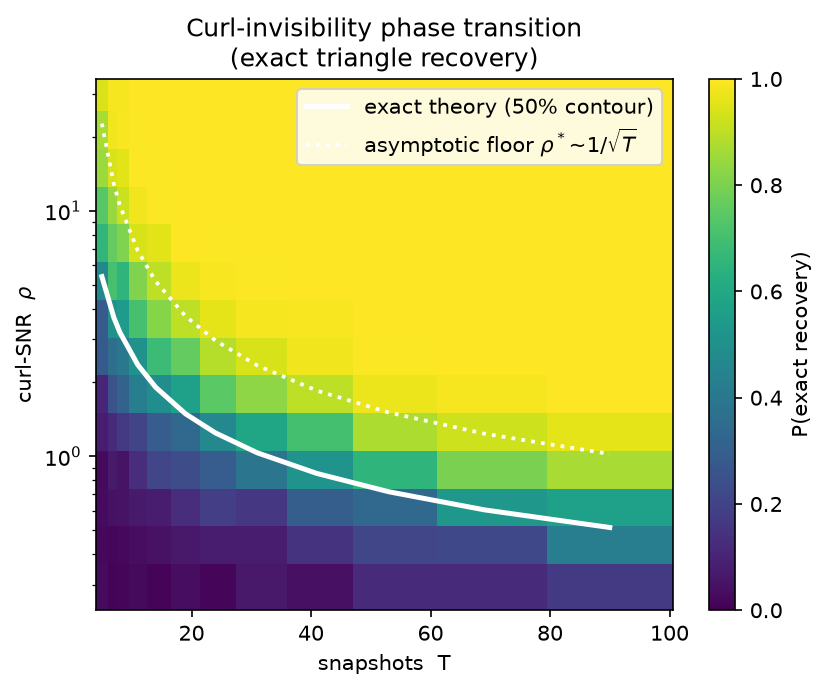
\includegraphics[width=0.92\linewidth]{phase_transition.png}
\caption{Curl-invisibility phase transition for exact triangle recovery. Colour is
empirical $P(\text{exact recovery})$; the solid line is the finite-sample theory,
the dotted line the $1/\sqrt T$ asymptotic floor.}
\label{fig:phase}
\end{figure}

\subsection{Confusability}
On an edge-sharing triangle strip (Fig.~\ref{fig:conf}), the naive curl-energy
detector fails and \emph{worsens} with $\rho$ due to leakage, while the whitened
detector of Theorem~\ref{thm:whiten} recovers the support and matches the
geometry-aware theory; a greedy baseline lies in between.

\begin{figure}[t]
\centering
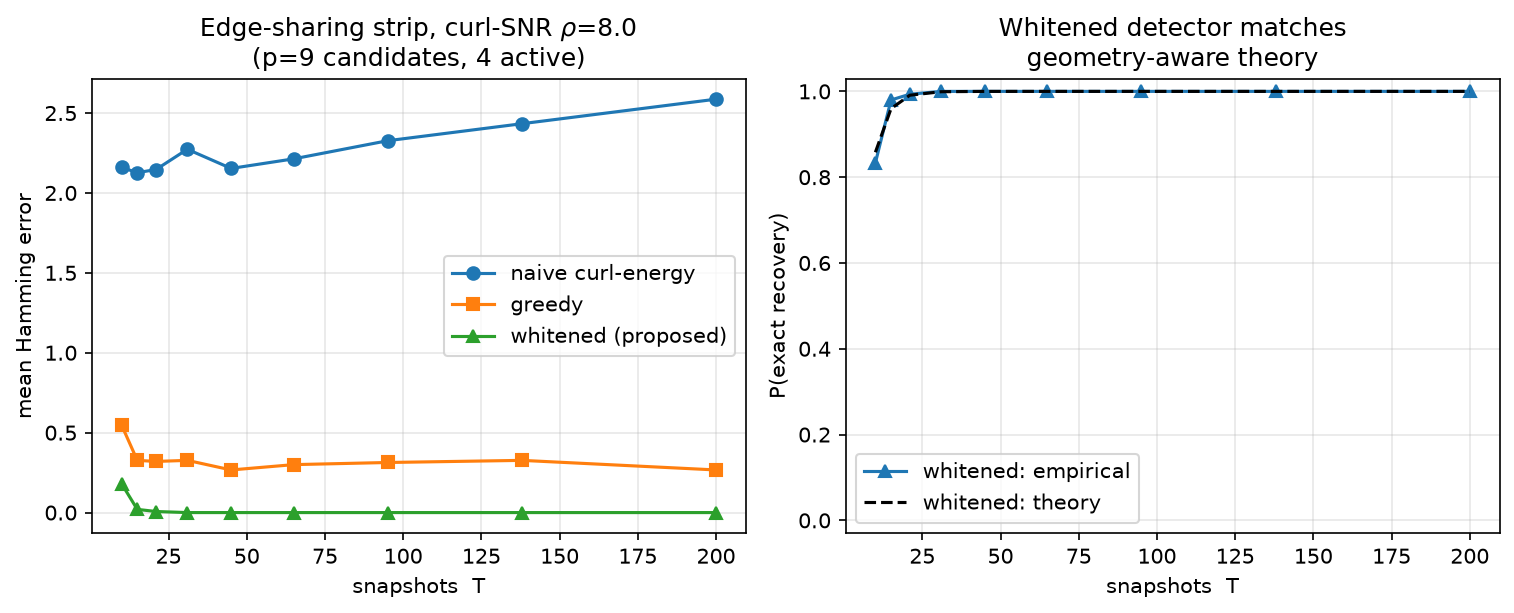
\includegraphics[width=\linewidth]{confusability.png}
\caption{Edge-sharing strip. Left: mean Hamming error vs.\ $T$; the naive detector
never recovers. Right: whitened detector matches the geometry-aware recovery law.}
\label{fig:conf}
\end{figure}

\subsection{Real foreign-exchange flows}
We form edge flows from $257$ trading days of ECB daily reference rates over nine
currencies (Fig.~\ref{fig:fx}). Both obstructions bind: (A) an arbitrage-free market
is a pure gradient, so its curl energy is $10^{-31}$ of its gradient energy---the
higher-order structure is invisible at any budget; (B) the complete currency graph
$K_9$ has only $28$ curl dimensions for $84$ candidate triangles, matching the $3/n$
law of Theorem~\ref{thm:rank}.

\begin{figure}[t]
\centering
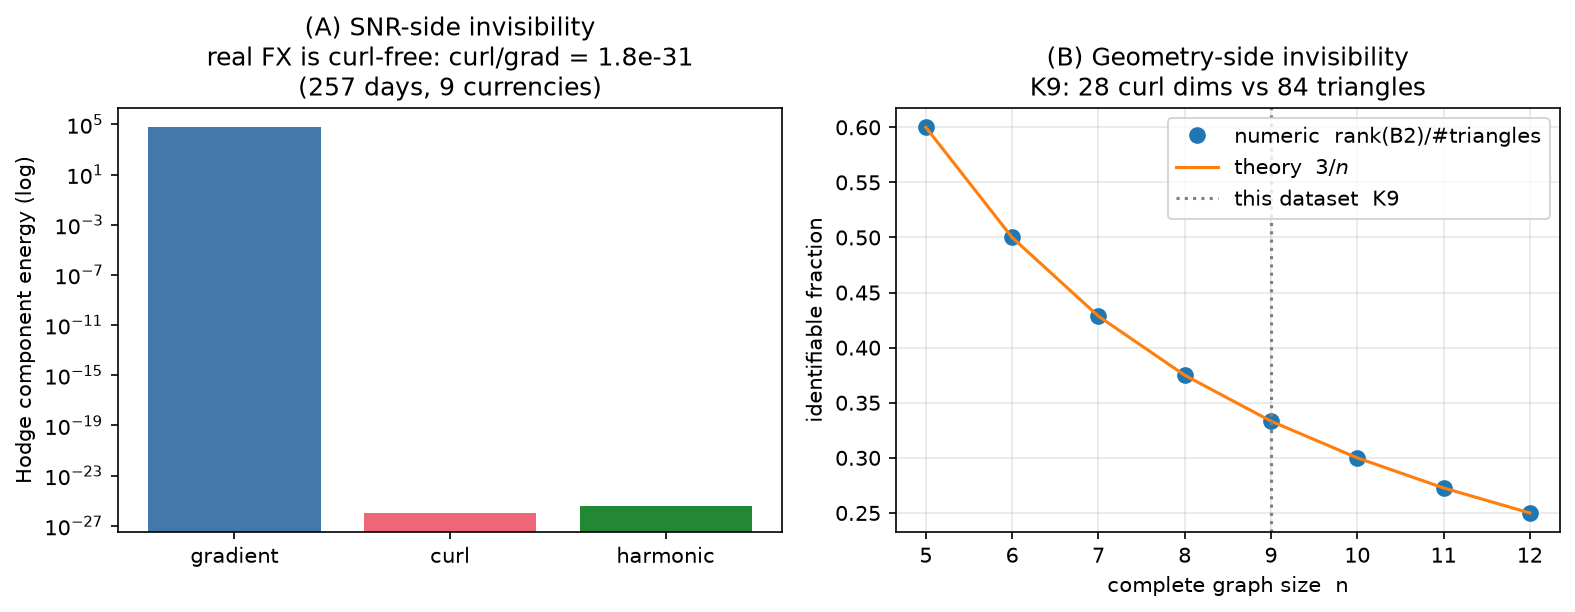
\includegraphics[width=\linewidth]{real_fx.png}
\caption{Real FX flows. (A) SNR-side invisibility: curl energy is machine-zero
relative to gradient. (B) Geometry-side invisibility: identifiable fraction $=3/n$.}
\label{fig:fx}
\end{figure}

\section{Conclusion}
We gave the first fundamental limits for identifying higher-order structure from
edge flows: a curl-invisibility phase transition, a geometry-aware whitened detector
that attains it, and a rank obstruction that no SNR can overcome. The results
delimit when the algorithmic TSP inference methods can succeed, and are borne out on
real data. Extending the converse to sub-Gaussian signals and to partial edge
sampling are natural next steps.

\bibliographystyle{IEEEtran}
\bibliography{refs}

\end{document}
